\begin{paper}{LB1}

\begin{header}
\author{Ludwig Boltzmann}
\title{On a medium whose mechanical characteristics lead to those specified by the Maxwell equations for electromagnetism.}

\makeheader

\end{header}

\section{Part I.}

We imagine a fine substance endowed with mass and inertia (but not with weight) and for brevity call it the ether. It shall permeate all bodies and also the so-called vacuum. We leave aside whether the properties we attach to it can be realized by a molecular structure and provisionally imagine the ether as a continuum, in the exact same sense that Kirchoff \?{used}{...} in the chapters on elasticity and hydromechanics of his lectures on mathematical physics which dealt with ponderable matter. We assume isotropy everywhere, and provisionally also exclude crystals. Where \?{direct}{gerade} electromotive forces are not \?{active}{thätig}, the ether should flow according to the same laws as an incompressible fluid; to the forces which affect such a fluid we should however add two more:

1. At each position (perhaps through the nearby ponderable matter, but also in the so-called vacuum) it experiences a resistance which is proportional to and directed against the velocity at this position. The work performed in this way should be transformed into heat (Joules).

2. At each position a torque acts on the ether volume element there, which is proportional to and directed against the \?{total twisting}{gesammten Verdrehung}. In this I completely follow Thomson's idea\footnote{Sir W. Thomson, Math. and phys. papers \textbf{3} article 99.}; the idea of a rotation of a volume element is to be understood in the sense used by Stokes and Helmholtz.\footnote{Stokes, On the Theories of the internal friction of fluids in motion etc., Trans. Cambr. Phil. soc. April 1845; Helmholtz, Ueber die Integrale der hydrodynamischen Gleichungen, welche Wirbelbewegungen entsprechen. Celle's Journ. \textbf{55}; Kirchoff, Tenth lecture on mechanics. Teubner 1883.}

Next we suppose that the ponderable matter is at rest and for any \?{piece of ether}{Aethertheilchens} with coordinates $x,y,z$ at time $t$ we denote the \?{translations}{Verschiebungen} by $F, G, H$ and the components of the velocity by $\varphi, \chi, \psi$ in the coordinate directions. Then
\nequ{1}{
a &= \ddy{H} - \ddx{G}\\
b &= \ddx{F} - \ddx{H}\\
c &= \ddx{G} - \ddy{F}
}
are \WTF{the doubled rotations} of the ether volume element found there. According to our assumption the volume element there is acted upon by the torque
\uequ{
\frac{a\d{\tau}}{2\pi\mu};
\frac{b\d{\tau}}{2\pi\mu};
\frac{c\d{\tau}}{2\pi\mu};
}
about the coordinate axes, whose work during the time $\d{t}$ is equal to:
\uequ{
\left(
\frac{a}{4\pi\mu}\cdot\ddt{a} + 
\frac{b}{4\pi\mu}\cdot\ddt{b} + 
\frac{c}{4\pi\mu}\cdot\ddt{c}
\right)\d{t}\d{\tau}.
}
Inside of a homogenous isotropic body $\mu$ is a constant value. If we choose a time where there would still be no electric or magnetic disturbances, so the field is found completely in the normal state at the start time, then the work completed from the start time until the time $t$ by the torque at volume element $\d\tau$ is:
\nequ{2}{
\frac{a^2+b^2+c^2}{8\pi\mu}\d\tau.
}
Here of course the coordinates $x,y,z$ of the ether-element are to be interpreted as variables; if they are to be to understood as fixed coordinates, then the coordinates $\varphi, \chi, 
psi$ could be understood as the velocity of the ether predominating at any time $t$ in the directions of the coordinate axes, so that one would have
\nequ{3}{
F=\int\limits_0^t\varphi \d{t},\quad
G=\int\limits_0^t\chi \d{t},\quad
H=\int\limits_0^t\psi \d{t}.
}
The rotation experienced by the volume element $\d\tau$ at the point $x,y,z$ during the time $\d{t}$ about the $x$-axis would then be equal to:
\uequ{
\frac{\d{t}}{2}\left(\dX\psi\dY{y} - \dX\chi\dY{x}\right)
}
and $a$ would be twice the sum of the rotations about the $x$-axis experienced by all volume elements passing through the point $x,y,z$ from the time 0 until $t$ \?{at the moment of the transit}{im Momente des Durchganges}. $b$ and $c$ would have analogous meanings with respect to the $y$- and $z$-axes.

Neither version leads, with stationary ether motion (electrostatics, electrodynamics and induction of stationary and nearly stationary electric currents, magnetism) nor with very small vibrations (light) to different equations. Other phenomena have not at this time been quantitatively compared with the equations.

If we further denote the density of the ether by $k/4\pi$, then the kinetic energy of the ether in the volume element $\d\tau$:
\nequ{4}{
\frac{k}{8\pi}\left(\varphi^2 + \chi^2 + \psi^2\right)d\tau.
}
\?{To get the equations of motion}{bloss um die Bewegungsgleichungen...zu erhalten} of the ether, we imagine arbitrary forces acting at every volume element $\d\tau$ with the components:
\uequ{
X\d\tau,\quad
Y\d\tau,\quad
Z\d\tau
}
where the work during the time $\d{t}$ is thus:
\uequ{
\left(
X\ddt{F} + X\ddt{G} + Z\ddt{H}
\right)\d{t}\d\tau.
}
Additionally in the associated volume element the work
\nequ{6}{
C\cdot\left[\left(\ddt{F}\right)^2 + 
\left(\ddt{G}\right)^2 +
\left(\ddt{H}\right)^2 +
\right]\d{t}\d\tau
}
is to be transformed into heat, so the equation of the \WTF{animating forces} reads
\nequ{7}{
0=\int\d\tau = \frac{1}{\mu}&\left(a\ddt{a} + b\ddt{b} + c\ddt{c}\right)\\
 + k&\left[\varphi \ddt{\varphi} + \chi\ddt\chi + \psi\ddt\psi \right]\\
 + 4\pi&\left(X\ddt{F} + Y\ddt{G} + Z\ddt{H}\right)\\
 + 4\pi C&\left[\left(\ddt{F}\right)^2 + \left(\ddt{G}\right)^2 + \left(\ddt{H}\right)^2\right],
}
where this integral ranges over the whole space. If there are different bodies there, then we will never think of the boundary surfaces as absolute discontinuities, but rather as transition layers within which the values of $\mu$, $k$ and $C$ transition continuously (if also quickly) from the inside of one to the inside of the other body.

For $\ddt{a}$, $\ddt{b}$ and $\ddt{c}$ we substitute the values from the equation (2) and partially integrate every term. According to the assumptions made there is no discontinuous surface on the inside, but at a great distance on the imagined outside surface of our space the $F$, $G$ and $H$ should vanish, so that all surface integrals vanish. Further, substituting for $\varphi$, $\chi$, $\psi$ their values from equation (1), then equation (7) goes over to
\nequ{8}{
\int\d\tau = & \ddt{F}\left[
   \dX{}\dY{y}\left(\frac{c}{\mu}\right)
 - \dX{}\dY{z}\left(\frac{b}{\mu}\right)
 + k\ddX{F}\ddY{t} + 4\pi C\ddt{F} + 4\pi X
\right]\\
+&\ddt{G}\left[
   \dX{}\dY{z}\left(\frac{a}{\mu}\right)
 - \dX{}\dY{x}\left(\frac{c}{\mu}\right)
 + k\ddX{G}\ddY{t} + 4\pi C\ddt{G} + 4\pi Y
\right]\\
+&\ddt{H}\left[
   \dX{}\dY{x}\left(\frac{b}{\mu}\right)
 - \dX{}\dY{y}\left(\frac{a}{\mu}\right)
 + k\ddX{H}\ddY{t} + 4\pi C\ddt{H} + 4\pi Z
\right] = 0.
}
Since the forces and accelerations, with the exception of course of those \?{up against obstacles}{von den Bewegungshindernissen herrührenden}, are independent of the velocities predominating at that instant, in this equation $\ddt{F}$, $\ddt{G}$, $\ddt{H}$ are considered at be independent and their coefficients must vanish separately. One can incidentally transform the variations of $F$, $G$ and $H$ into proper variations by giving the quantities $X,Y,Z$ very large values during a very brief interval of time. (cf Maxwell, On physical lines of force, Scient. Pap. I. p. 475, equation 53. Phil. Mag. (4) vol. 21).

If we then put, for brevity:
\nequ{9}{
f=-\frac{4}{4\pi}\cdot\ddt{F};\quad
g=-\frac{4}{4\pi}\cdot\ddt{G};\quad
h=-\frac{4}{4\pi}\cdot\ddt{H}
}
\nequ{10}{
p=-C\ddt{F};\quad
q=-C\ddt{G};\quad
r=-C\ddt{H}
}
\nequ{11}{
u=p+\ddt{f};\quad
v=q+\ddt{g};\quad
w=r+\ddt{h},
}
then we obtain:
\nequ{12}{
4\pi\cdot u &= \dX{}\dY{y}\left(\frac{c}{\mu}\right) - \dX{}\dY{z}\left(\frac{b}{\mu}\right)\\
4\pi\cdot v &= \dX{}\dY{z}\left(\frac{a}{\mu}\right) - \dX{}\dY{x}\left(\frac{c}{\mu}\right)\\
4\pi\cdot w &= \dX{}\dY{x}\left(\frac{b}{\mu}\right) - \dX{}\dY{y}\left(\frac{a}{\mu}\right)
}
which coincides exactly with the equations that Maxwell found for electric and magnetic phenomena in resting bodies. (cf my lectures on Maxwell's theory, l.t.z. Barth. 1891. p.84 art. 88.)

These equations could be found directly by the following method, also already applied by Thomson l.c. in a similar manner. Let the volume element $\d\tau$ be a parallelepiped where one corner has the coordinates $x,y,z$ while the others have larger coordinates about $\xi$ \?{resp.}{resz.}, $\eta,\zeta$. Hence there is a torque about the $x$-axis:
\uequ{
m=\frac{b\xi\eta\zeta}{2\pi\mu}.
}

The volume element is however connected with the surrounding ones so that it cannot be detached and this rotation \WTF{can} be carried out without this \?{turning along with it}{mitzudrehen}. It will hence have to be subject to tangential forces from the surrounding pieces of the ether on the four boundary surfaces which are parallel to the $x$-axis, which together supply the equal torque. If we assume in contrast to the usual behavior of elastic bodies that here changes in the angle of the parallelepiped do \textit{not} evoke considerable elastic forces, so that the usual tangential forces of \?{elasticity}{der Elasticit\"atslehre} are close to zero, then the torque will be distributed uniformly over both surfaces. On the one surface $\phi$ from $\xi\eta$, which makes a right angle with the $x$-axis there is a force $m/2\zeta$ in the positive $x$-direction, on the opposite surface $\phi'$ there is one in the negative $x$-direction. These forces will act on the surfaces dividing every two volume elements and naturally change in intensity from point to point in space. Since however $\phi'$ and $\phi$ are distinguished in that $z$ is greater than $\zeta$, the following forces act on the latter surface \WTF{mit Beachtung des Kleinen 2. Ordnung}:
\uequ{
\frac{1}{2\zeta}\left(m + \ddz{m}\zeta\right).
}
Then both forces together supply
\uequ{
\frac{1}{2}\cdot\ddz{m} = \frac{\xi\eta\zeta}{4\pi}\cdot\ddz{\frac{b}{\mu}}
}
in the $x$-direction. The resultant is totally analogous:
\uequ{
-\frac{\xi\eta\zeta}{4\pi}\ddy{\frac{c}{\mu}}.
}
Subtracting the frictional resistance $C\ddt{F}$ from these molecular forces and setting the thus-obtained total force equal to the mass $k\xi\eta\zeta/(4\pi)$ multiplied by the acceleration in the $x$-direction and finally multiplying by $4\pi/(\xi\eta\zeta)$ then the above equation immediately follows:
\uequ{
k\ddX{F}\ddY{t}+4\pi C\dX{F}\dY{t} = \ddz{\frac{b}{\mu}} - \ddy{\frac{c}{\mu}}.
}
Th)e fundamental equations of electromagnetism for moving bodies are found by taking $x,y,z$ not as the coordinates of a fixed point in space, but rather a point of a ponderable body that follows along with its motion. In spaces where there is no ponderable matter every arbitrary \?{compatibile}{damit verträgliche} motion can be ascribed to the ether. There motions must be \?{superimposed}{superponiren} with the. motions described. earlier. (c.f. Hertz on the foundations of electrodynamics in moving bodies. Wied. Ann. vol 41, p.369, 1890; Ges. Abh. p.256).

As is seen, the entire proof is based on the expressions (2), (4), (5), (6) for the energy of the ether. (2) can now also be obtained another way, \WTF{as by the previously superimposed torque}. The ether is imagined in an isotropic medium as a homogenous, isotropic elastic body and $F,G,H$ as the displacements of a piece of it, the energy of the elastic forces is then, as is known:
\nequ{13}{
A=K\left[
\left(\ddx{F}\right)^2 + \left(\ddy{G}\right)^2 + \left(\ddz{H}\right)^2 
+ \frac{1}{2}\left(\ddz{G} + \ddy{H}\right)^2\right.\\
\left. + \frac{1}{2}\left(\ddx{H} + \ddz{F}\right)^2
+ \left(\ddy{F} + \ddx{G}\right)^2
+ \theta\left(\ddx{F} + \ddy{G} + \ddz{H}\right)\right]
}
(cf Kirchhoff, 11th lecture on mechanics. 3rd edition p.122.)

We will set $\theta=-1$ and every term of the form
\uequ{
\int\d\tau K\ddx{F}\ddy{G}
}
is first partially integrated with respect to $x$ and then $y$. If $K$ has the same value everywhere, the separating surfaces of two bodies has no mathematical discontinuity and $F,G,H$ vanish on the imagined boundary surface at infinity surrounding the whole system under consideration, then the surface terms also vanish, and equation (13) is transformed into
\uequ{
A = \frac{K}{2}\left[
\left(\ddy{H} - \ddz{G}\right)^2 + 
\left(\ddz{F} - \ddx{H}\right)^2 + 
\left(\ddx{G} - \ddy{F}\right)^2
\right],
}
which coincides with expression (2) when $K=1/(4\pi\mu)$. Then the Maxwell equations would likewise follow. Here it is of course to be noted that for a fixed body with a \?{freier im Endlichen liegenden Oberfläche}{free surface at infinity}, $\theta$ cannot have a negative value. Only with an everywhere unbounded body, like the ether, are negative values of $\theta$ permissible, at least when dealing with a dynamic illustration, as in this case\footnote{The state required by $\theta=-1$, which Thomson l.c. calls \?{quasistable}{quasilabilen}, was discovered by Loschmidt in his writing on the nature of the ether, Vienna at Gerold \& Sohn 1862, cf Forschritt der Physik, 1862, p.68.}. If one additionally ascribes incompressability to the ether, then eo ipso
\uequ{
\ddx{F} + \ddy{G} + \ddz{H} = 0
}
and the factor $\theta$ \?{for these values}{welcher bei dieser Gr\"osse steht}, \WTF{gleichg\"ultig, } and hence the Maxwell equations arise not merely for $\theta = -1$, but rather for every arbitrary value of $\theta$. Namely this also applies for $\theta=\infty$, which has incompressibility as a consequence. For other values of $\theta$ a generalized Maxwell theory would be obtained, like those Helmholtz derived from the action-at-a-distance equations. The blatant contradiction-
between the existence of such magnetizable bodies as iron and the assumption that $K$ is equal in all bodies can, I believe, be removed by the supposition that the high magnetizability of iron is not caused by the predominance of a smaller value of $K$ in its interior, but rather by a molecular magnet already present in it. i.e. small electric currents of unchanging intensity \?{which is only directed to the magnetization}{die bei der Magnetisirung bloss gerichten werden}.

Here too is something to note. The ether, which we initially assumed to be an incompressible fluid, will \?{attain}{beigelegt} new properties of a fixed substance. It must behave like a fixed body with respect to certain forces, like a fluid with respect to other. \?{There are analogies for it in ponderable bodies}{Analogien daf\"ur an ponderabeln K\"orpern fehlen nicht}. One thinks of Tresca's investigation on the outflow of fixed bodies which are forced through openings with great pressure. In such bodies, despite the applicability of the equations of elasticity inside certain bounds, the displacements $F, G, H$ can assume arbitrarily large values. The theory of these bodies is apparently of the greatest importance for research into the nature of the ether. Cf Stokes, on the nature of the ether, how it \?{emerges from}{sie sich...ergibt aus} the aberration. Phil. Mag. July 1846. Scient. pap. vol. I, p.153. Incidentally there are still difficulties, that our equations supply $k$ \WTF{with the time changeable} while the assumption of incompressibility would again introduce foreign pressure forces into the Maxwell theory. Here I will include some more investigation as to whether this hypothesis does not come into conflict in quantitative relations.

Let a homogenous isotropic medium, e.g. air, be  given. Let it have a very small value for $C$; for a given value of the velocity
\uequ{
\omega = \sqrt{\varphi^2 + \chi^2 + \psi^2}
}
then let the heat converted into \?{energy}{lebendige Kraft} in a unit of time and volume of the ether $C\omega^2$ be very small. Such a body is called a poor \?{elecrical conductor}{Electricitätsleiter}, since with a given current strength $\delta=C\omega$ the Joule heat that arises is inversely very large $\delta^2/C$. Let:
\uequ{
F=\ddx{W};\quad G=\ddy{W};\quad H=\ddz{W}; V=\ddt{W}.
}
The pressure at any point is then
\uequ{
p+p_0-\frac{k}{8\pi}\left[\left(\ddx{V}\right)^2
\left(\ddy{V}\right)^2 = \left(\ddz{V}\right)^2
\right].
}
The total force $X$ acting on a particle in the ether in the direction of the $x$-axis is
\uequ{
X=\int p\D{s} \cos{(n,x)} = \iint p\D{y}\D{z} = \int \ddx{p} \D\tau,
}
where $\tau$ is a volume element, $\d{s}$ is a surface element on the body, $n$ is the normal from the latter. The substitution of the value for $p$ gives
\uequ{
X=-\int\D\tau \frac{k}{4\pi}\left[\ddx{V}\cdot\ddX{V}\ddY{x}
+ \ddy{V}\ddX{V}\dY{x}\cdot\dY{y} + \ddx{V}\cdot\ddX{V}\dY{x}\dY{z}\right]
}
and partial integration gives
\uequ{
X=\int k \frac{\d\tau}{4\pi}\ddx{V}\Delta V.
}
Setting $\Delta V = -4\pi\epsilon$ and considering only the coordinates $\xi\eta\zeta$ of the electrical mass $\epsilon\D\tau$ as variable, one obtains
\uequ{
X=-k\dX{}\dY\xi\int\epsilon V\D\tau.
}
(Cf Maxwell, Scient. pap. vol. I. p.497.)

Here we shall only treat one very special example in a very direct manner. In the medium described above, there are two like charges. The first should only differ infinitely little from a sphere with center $A$ and radius $o$\sic, the second only infinitely little from a sphere with center $B$ and radius $\varrho'$. \?{We select $A$ for the starting coordinate point and pull the negative abscissa towards $B$}{Wir w\"ahlen $A$ zum Coordinatenanfangspunkt und ziehen die negative Abscissenaxe gegen $B$ hin}. The length $AB=\gamma$ should be very large with respect to the two radii $\varrho$ and $\varrho'$. If we again put
\uequ{
F=\ddx{W};\quad
G=\ddy{W};\quad
H=\ddz{W},
}
then it is well known that to this problem corresponds the solution
\uequ{
W=\frac{M}{r}+\frac{N}{s},
}
where $M$ and $N$ are functions of the time, $r$ and $s$ the distances of the point to with the coordinates $x,y,z$ of the reference point, from $A$ resp. $B$. Further:
\uequ{
\varphi = \ddx{V};\quad
\chi = \ddy{V};\quad
\psi = \ddz{V};
}
where $V$ is the derivative of $W$ by time, so
\uequ{
W=\frac{M'}{r}+\frac{N'}{s},
}
where
\uequ{
M'=\ddt{M};\quad N'=\ddt{N}.
}
This gives $a=b=c=0$ everywhere. Hence it follows from equation (12) that 
\uequ{
u=p+\ddt{f} = -C\varphi - \frac{k}{4\pi}\ddt{\varphi} = 0,
}
so
\nequ{14}{
M'=\alpha\exp{-\frac{4\pi Ct}{k}}\\
N'=\beta\exp{-\frac{4\pi Ct}{k}}
}
$\alpha$ and $\beta$ are constants.

The volume of ether that the first body passes through in the time $\d{t}$ is
\uequ{
4\pi\varrho^2\frac{M'}{\varrho^2}\d{t};
}
everything else can be ignored as infinitely small. The whole ether that the first body passes through from time 0 to time $\infty$, \?{with which it was charged, has the following volume after the particle leaves}{womit dieser also geladen war, hat nach dem Ausstr\"omen das Volumen}:
\nequ{15}{
\Omega = 4\pi\cdot\int\limits_0^\infty M'\D{t} = k\frac{\alpha}{C},
}
since $k/(4\pi)$ is the density of the ether after the \WTF{outflow}. (The body itself could be composed of any ponderable mass, \?{where we think of the ether being arbitrarily condensed by any (chemical) force}{worin wir uns den Aether durch irgend welche Kr\"afte beliebig verdichtet denken}.)

The mass of the ether \WTF{with which the first particle was charged}{womit der erste K\"orper geladen war} is then
\nequ{16}{
m=\frac{k^2\alpha}{4\pi C}.
}
For the second body the same quantity has the value
\uequ{
\frac{k^2\beta}{4\pi C}.
}
We will now seek the total force $X$ acting on the first body as a consequence of the ether's pressure. This is constantly sent out through interior ether forces normal to its surface. If it is absolutely spherical, then the ether motion specified by the above formulae would have to be modified a little, so that the ether radiation appears everywhere the surface of the body. It simplifies the calculation when inversely lets the form of the body deviate from the spherical so that its surface is every perpendicular to the ether current defined by the above equations; i.e. the equation
\uequ{
\frac{\alpha}{r}+ \frac{\beta}{s} = c
}
is satisfied, where $c$ is a constant.

Let $x,y,z$ be the coordinates of a point of the body's surface; if we put
\uequ{
y^2+z^2=\eta^2,
}
then
\uequ{
\frac{\alpha}{r} + \frac{\beta}{\sqrt{\gamma^2 + 2\gamma x + x^2 + \eta^2}} = c,
}
and so, since $\gamma$ is large with respect to $r$:
\nequ{17}{
\frac{\alpha}{r} = e + \frac{\beta x}{\gamma^2}.
}
The pressure at the point with coordinates $x,y,z$ is (again, ignoring the infinitely small higher order values) is
\uequ{
p=p_0 - \frac{k}{8\pi}\left(\frac{\alpha^2}{r^4} + \frac{2\alpha\beta x}{r^3\gamma^2}\right).
}
$p_0$ denotes the pressure at a very large distance. If in the first term in the brackets we insert for $1/r^4$ its value from equation (17) and then in the terms of lowest order in $c$ we again insert its approximate value $\alpha/r$, then it follows that
\uequ{
p=p_0 - \frac{k}{4\pi}\left(\frac{c^2}{\alpha^3} + \frac{6\alpha\beta x}{r^3\gamma^2}\right).
}
All points of the body for which $x$ lies between $x+\d{x}$ and $\eta$ lies between $\eta$ and $\eta+\d\eta$ form a band of the surface
\uequ{
2\pi\eta\sqrt{\d{x}^2 + \d\eta^2}.
}
The pressure acting on this band has the component $-2\pi p\d\eta$ in the direction of the positive abscissa. Since $\eta\d\eta$, integrated over the whole body, is equal to zero, so the first two constant terms in the expression for $p$ vanish, and the total force acting on the first body in the direction of the abscissa is
\uequ{
X=\frac{3k\alpha\beta}{2\gamma^2}\cdot\int\frac{x\eta\d\eta}{r^3}.
}
Here the body can again be considered a sphere and
\uequ{
x&= r\cos\vartheta\\
\eta &= r\sin\vartheta
}
where, since $r$ is constant, one obtains
\uequ{
X=\frac{3k\alpha\beta}{2\gamma^2}\cdot\int\limits_0^\infty
\cos^2\vartheta\sin\vartheta\D\vartheta = \frac{k\alpha\beta}{\gamma^2}.
}
Now let the dielectric be such a poor conductor that the charge sinks from $1$ to $1/e$ ($e=2.718\dots$) in $T$ days. Then
\uequ{
\frac{4\pi C}{k} = \frac{1}{24\cdot 60\cdot 60\cdot T\unit{sec}},\quad
C=\frac{k}{10^6\cdot T\unit{sec}}.
}
Further, each of the charged spheres have radius $R$ and start charged with $30,000\unit{V}$. One volt is, in electromagnetic units, the potential
\uequ{
\frac{10^8\sqrt{\gram\,\unit{cm}^3}}{\unit{sec}^2};
}
in electrostatic units
\uequ{
\frac{\sqrt{\gram\,\unit{cm}}}{300\unit{sec}}.
}
Since the potential of a sphere is the \?{total electricity}{Electricit\"atsmenge} divided by the sphere's radius, the \WTF{total electricity} present on each sphere is, measured in static units:
\uequ{
\epsilon = \frac{100R\sqrt{\gram\,\unit{cm}^3}}{\unit{sec}}\unit{V}.
}
The force with which the spheres are repelled is $X=\epsilon^2/\gamma^2$ and comparing this with the value of $X$ found it follows that
\uequ{
\alpha &= \frac{\epsilon}{\sqrt{k}} = \frac{100}{\unit{sec}}\unit{V}
R\sqrt{\frac{\gram}{\cm^3}}{k}, \text{so:}\\
\Omega &= 10^8\volts\cdot T\cdot R\sqrt{\frac{\gram\,\cm^3}{k}};\\
m &= \frac{10^8}{4\pi}\volts\cdot T\cdot R\sqrt{k\cdot \gram\,\cm^3}.
}
If we set the density of the ether to $10^{16+2h}$ times smaller than that of water, then
\uequ{
k &= 10^{-16+2h}\frac{\gram}{\cm^3}\cdot 4\pi,\textit{then:}\\
\Omega &= \frac{10^{h+16}}{\sqrt{4\pi}}\volts TR\cm^3;\quad
m=\frac{10^{-h}}{\sqrt{4\pi}}\volts TR\gram.
}

Thomson found $10^{-22}\gram\,\cm^{-3}$for the lower limit of the density of the ether. If it was actually equal to this lower bound, then one would have $h$ equal to about $3.5$, $m=\volts TR/(11000\gram)$. If $R=1,T=1$ for the medium where the posited one-$\cm$ radius sphere is found, i.e. the charge would decrease by one part in 2,718 in one day, then for $V=1$, i.e. with a charge of $30,000$ volts, then there is already $1/(11000\gram)$ brought into it, or taken out of it. Now there are undoubtedly media where $T$ is much larger, so that $m$ is still greater. One must only imagine that for the enormous charge we have assumed that the laws followed by electrical conduction and distribution are essentially complicated, so that the applicability of the simple linear Maxwell equations is questionable. So if this number lies at all close to the limit, then in my view it cannot be claimed that it contradicts experiment. The values which follow for the speed of the ether are more dubious.

With a view to further elucidation of our mechanical analogy we consider the same dielectric as above (air). There will be however various bodies in it in which $k$ and $C$ have different values. In the air and in all bodies \?{where $C$ is small of the same order of magnitude}{worin $C$ klein von derselben Grössenordnung ist}, $\varphi, \chi, \psi$ will remain finite for a long time, otherwise, since everything is almost stationary, their differential quotients with respect to time, as well as $p,q,r$ and $u,v,w$, will soon become very small. Hence according to equation (12)
\uequ{
\frac{a}{\mu}\d{x} + \frac{b}{\mu}\d{y} + \frac{c}{\mu}\d{z}
}
becomes a total differential $\d{W}$, i.e. the magnetic forces have a potential. Further it follows from equation (2) that
\uequ{
\ddx{}\left(\mu\ddx{W}\right) +
\ddy{}\left(\mu\ddy{W}\right) +
\ddz{}\left(\mu\ddz{W}\right) = 0
}
Since $W$ and $\mu$ is everywhere continuous and the first quantity is equal to zero at infinity, it follows that
\uequ{
W=a=b=c=0.
}
The upper equation is namely the condition that
\uequ{
\iiint \mu\D{x}\D{y}\D{z}\left[\left(\ddx{W}\right)^2 + \left(\ddy{W}\right)^2 + \left(\ddz{W}\right)^2\right]
}
is a minimum, which is only satisfied for $W=0$.

In this representation it is seen why magnetization happens so that the magnetic energy, i.e. the sum of the square of the volume element multiplied by $\mu$, is a minimum, as well as other similar minimum laws. (cf Stefan, Vien. Sitzungber. vol 99 p.319, 1890.)

If Ampere's molecular currents were in individual bodies then in these and on their surfaces $u,v,w$ would not equal zero. Hence one would get a magnetic potential different from zero. Very rapid changes of it with the time (magnetic current) would give rise to electrical forces, as have of course not yet been observed. We will however exclude such cases here and set $a=b=c=0$ everywhere. Then it follows from equation (2) that
\uequ{
\varphi\d{x} + \chi\d{y} + \psi\d{z}
}
likewise $\d{V}$ is a total differential, so that the electrical forces also have a potential. We imagine the dividing surface between the two bodies as a very thin, but continuous transition layer in which the same conditions are fulfilled that we have assumed everywhere. Since equations (2) must also be fulfilled inside this transition layer, it is found in the well known manner of differentiating with respect to $t$ and choosing the abscissa axis to be normal to the transition layer that the differential quotient of $V$ with respect to a direction tangential to the transition layer must have the same value on both sides of it. \?{The ether mass passing through the unit surface $dv$ of the transition layer}{Die durch die Flächeneinheit $dv$ der Uebergangsschicht hindurchgebende Aethermasse} is
\uequ{
\frac{k}{4\pi}\cdot\frac{V\d}{\d{n}},
}
where $n$ is the direction normal to the transition layer. Since the same ether mass must occur on both sides, this expression must have the same value on both sides. Those are the old well-known boundary equations at the dividing surface of two dielectrics.
-
If in a body $C$ had a greater value, $V$ decreases more quickly (the electric \?{effect}{Nachwirkung}, electric absorption). If $C$ has a very large value, i.e. the body is a conductor, then $V$ must soon become constant. The ether current then surrounds the body in question like water around a fixed submerged body. The modification in the value of $V$ brought about this way is called the electrification of the submerged body by induction. This modification can also be thought of as the motion of the ether is made by the emission from the ether on the positive side of the body and an influx on the negative without a conductor being present, by the \WTF{Beschaffenheit} that the motion of the ether is made everywhere tangential to the surface of the body. In the body itself is only a very weak current which causes the slow decreas of the electrical induction which is required by the gradual decay of the electricity in the originally charged body. In general terms this would be the idea of the so-called electrostatics.

To provide an idea of the motion of the ether with stationary electric currents, we will consider an infinitely long straight cylinder of radius $\varrho$ and \?{where the positive electrical current flows from the direction of the positive axis}{der in Richtung der positiven Abscissen vom positiven electrischen Strome durchflossen wird}. The electrostatic potential that is necessary to drive such a current is infinite at an infinite distance from the axis. In the old action at a distance theory this causes little harm since the electrostatic and electrodynamical phenomena are considered to be completely separate. It must be seen as an advantage of the new theory that such a separation is not needed at all.

In order to make the electrostatic potential finite we could take the cylinder to be surrounded with a hollow cylinder of a very large radius $R$, which is attached to the earth and without electromotive force. Let $A/C$ be the current density in the massive cylinder, so the same $F$ must contain the term $-At$. Since we are dealing with a conductor, we set $k=0$ and it follows from equation (80) in my "Lectures on Maxwell's theory", and which indeed can also be easily from the equations developed here:
\uequ{
F=-At - \pi\mu ACr^2,\quad G=H=0
}
where $r=\sqrt{y^2+z^2}$ is understood to be the distance of the points from the axis of the cylinder. From this it follows in the interior of the massive cylinder:
\uequ{
a=0;\quad b=-2\pi\mu ACz;\quad c=\pi\mu ACy.
}
There is a dielectric (air) between the massive and hollow cylinders. It should have for $\mu,C,k$ the values $\mu',C',k'$, where $C'$ is very small. On the dividing surface one must have
\uequ{
a=a'\quad \mu b = \mu' b' \quad \mu C = \mu' C'\quad F=F'\\
C\ddt{G} = \frac{k'}{4\pi}\ddt{G'}\quad
C=\ddt{H'} = \frac{k'}{4\pi}\ddt{H}.
}
The just-cited equation (80) here gives
\uequ{
\Delta F = \Delta G = \Delta H = 0.
}
So next:
\uequ{
F=-A\left(\frac{t}{l\frac{\varrho}{R}} + 2\pi\mu'C\varrho^2\right)
l\frac{r}{R} + \pi AC\varrho^2\left(2\mu'l\frac{\varrho}{R} - \mu\right),
}
where $l$ denotes the natural logarithm. Further since $a,b,c$ cannot increase to infinity, because infinite forces would be \?{needed}{geweckt}, in the dielectric the part of
\uequ{
F\d{x} + G\d{y} + H\d{z}
}
containing $t$ must be a differential, from which it follows that
\uequ{
G = -\frac{Atxy}{r^2 l \frac{\varrho}{R}}\\
H = =\frac{Atxz}{r^2 l \frac{\varrho}{R}}
}

The quantity
\uequ{
\frac{gy + hz}{r-\varrho} = -\frac{k}{4\pi\varrho}
\left(y\ddt{G} + \ddt{H}\right) = \frac{Ax}{l\frac{\varrho}{R}}
}
is what is called the surface density of the free electricity on the surface of massive cylinders
\uequ{
\int\left(\ddt{F}\d{x} + \ddt{G}\d{y} + \ddt{H}\d{z}\right)
 = -\frac{Ax}{l\frac{\varrho}{R}}l\frac{r}{R},
}
which is its potential function.

For electrostatic measurement in the standard medium $k=1$. It would be independent of $R$ if 🏃🏻‍♀️two cylinders with equal composition flowing in opposite directions, whose axes are $y=0,z=p$ and $z=-p$ were present
which have zero electrostatic potential for $x=0$. If then
\uequ{
r = \sqrt{y^2 + (z-p)^2} \text{ and } s=\sqrt{y^2 + (z+p)^2}
}
are the distances of a point from the first resp. second axis, and if the radius $\varrho$ of both cylinders is small with respect to $p$, then in the first cylinder
\uequ{
F = -At - \pi\mu ACr^2; \quad G=H=0;\\
a=0; b=-2\pi\mu AC(z-p); \quad c=2\pi\mu ACy;
}
in the second
\uequ{
F = At + \pi\mu ACr^2; \quad G=H=0;\\
a=0; b=-2\pi\mu AC(z+p); \quad c=2\pi\mu ACy
}
and in the surrounding dielectric
\uequ{
F&=\left(-\frac{t}{l^2\frac{p}{\varrho}} + 2\pi\mu'C\varrho^2\right)
Al\frac{s}{r} - \pi AC\varrho^2\left(2\mu' l^2 \frac{p}{\varrho} + u\right);\\
&G = \frac{Atxy}{l^2\frac{p}{\varrho}}\left(\frac{1}{r^2} - \frac{1}{s^2}\right); \quad
H = \frac{Atx}{l^2\frac{p}{\varrho}}\left(\frac{z-p}{r^2}-\frac{z+p}{s^2}\right);\\
&\quad a=0; b=-w\pi\mu'C\varrho^2\left(\frac{z-p}{r^2}-\frac{z+p}{s^2}\right);\\
&\quad\quad c=2\pi\mu C\varrho^2 y\left(\frac{1}{r^2}-\frac{1}{s^2}\right).
}
\subsection*{Supplement}

I would like to permit myself to append the following, admittedly disconnected remarks.

1. Herr A. Sommerfeld has\footnote{\citeauthor{Sommerfeld}, \citepub{Wied. Ann.} \citevol{46}. \citepage{p.139}. \citeyear{1892}.} has conversely attempted to set the electrical forces proportional to the torques $U,V,W$ of the magnetic fields with respect to the velocity components $u,v,w$ of a piece of the ether. If $\xi, \eta, \zeta$ are its displacements at time $t$, then $u=\d\xi:\d{t}$, $2U = (\d\zeta:\d{y} - \d\eta:\d{z})$. That one can in general get by in this manner, offers an interesting illustration of the reciprocity between electricity and magnetism\footnote{Cf besides Maxwell, among others \citeauthor{Rowland} \citepub{Amer. Journ. of Math.} \citevol{II}\citepage{354}\citeyear{1879}.\citevol{III} \citepage{89} \citeyear{1880}.} as well as the fact that all mechanical hypotheses, if they only satisfy certain general conditions, must lead to the electromagnetic equations\footnote{Cf. my lectures on the Maxwell el-theory. Barth 1891.}. But in specific cases difficulties could enter. So it seems to me that in Herr Sommerfeld's view a uniformly-electrified sphere is impossible. If we draw an arbitrarily small circle on the sphere, then we must have
\uequ{
\int\left(\xi\d{x} + \eta\d{y} + \zeta\d{z}\right) = 
\int\d\nu\left[\left(\ddy{\zeta} - \ddz{\eta}\right)\right.\cos{(nx)}\\
\left.\left(\ddz{\xi} - \ddx{\zeta}\right)\cos{(nx)} +
\left(\ddx{\eta} - \ddy{\xi}\right)\cos{(nz)}\right].
}
There the first integral is over the circumference of the small circle, the second over the whole spherical surface, with the exception of the surface enclosed by the circle. According to Herr Sommerfeld the \?{expression in the square brackets}{eckigeinklammerte Ausdruck} must be zero inside the sphere, but on the outside on its outer surface it is equal to a finite constant. So, the left side of the equality sign, when the small circle is drawn very close to (but outside) the sphere, must also be finite. So there must be at least one infinitely narrow tube \?{outwards from the sphere}{von der Kugel weg nach aussen} inside which entirely different behavior reigns. Since this applies at magnetic and solenoid poles but not at charged spheres, Sommerfeld's interpretation seems less likely to me.

Additionally, Herr Sommerfeld has waived the advantages offered by considering the discontinuities as very fast but not infinitely fast transitions by assuming that they do not satisfy his equation (2c), which is a consequence of his definition of $U,V,W$, and does not say what these quantities mean if the differentiations used in their definitions were not allowed.

2. If one sets before himself the task, following Herr Hertz's procedure\footnote{\citepub{G\"ott. Nachr.} \citedate{March 19th 1890}. \citepub{Wied. Ann.} \citevol{40} \citepage{577}. \citetitle{usbreit. d. el. Kraft.} \citeyear{1892}.}, of setting up the equations of electromagnetism in the simplest form without a mechanical basis, then the number of \?{auxilliary assumptions}{Hülfsvorstellungen} can be reduced by half by only considering the three electrical forces $F,G,H$ and the equation determining them as given according to experiment. This latter reads, for homogenous bodies,
\uequ{
k\ddX{F}\ddY{t} + 4\pi l \ddt{F} = \nu \bracket{\Delta F - \ddx{}\paren{\ddx{F} + \ddy{G} + \ddz{H}}}
}
but for inhomogeneous bodies there is also the term
\uequ{
\paren{\ddz{F} - \ddx{H}}\ddz{\nu} + \paren{\ddx{G} - \ddy{F}}\ddy{\nu}
}
The hypotheses expressed in these four lines suffice to explain the electromagnetic phenomena in isotropic resting bodies. The boundary layers will always be considered to be continuous, if arbitrarily rapidly changing, magnets as solenoids, iron and steel as aggregate revolving resp fixed small currents\footnote{On the introduction of such movable and fixed small currents in the Maxwell theory cf \citepub{Verhandl. Gesellsch. der Natur forscher} \citeyear{1891}.}, which all can be determined by the variables $F,G,H$ and their differential quotients, while the notation $\d{H}:\d{y} - \d{G}:\d{z}$ etc by individual symbols only serves to simplify the formulae.

3. The remarks on page 86 suggested considering as an analogy to the ether a body for which the equations apply, which I have put forward in two essays on the theory of elasticity\footnote{\citepub{Wien. Sitzungsber.} \citevol{70} \citedate{October 8th 1874}, \citevol{6}, \citedate{December 6th 1877}.}, and where I maintain the notation applied there with the same meaning, and only note the consequences. One could also interpret in this way my formulae, which incidentally only permit the Maxwell transformations\footnote{\citeauthor{Maxwell}, \citepub{Scientific papers II}, \citepage{p.623}.} when Maxwell's series converge, which e.g. never happens if the deformation ever differed from zero but then was zero for a finite time.

We \?{plot}{tragen...auf} the time from $-\infty$ until the time in question $t$ on the abscissa $OT$ in figure 1 and divide it into infinitely many differentials. Over each time we plot the values of $p=dv:dz - dw:dy$ found there, multiply them with the relevant time differentials\?{and likewise with a factor also plotted above if}{und noch einem ebenfalls darüber aufgetragenen Faktor}. The sum (integral) of these products is then the value of $T_1$ at the time in question. The endpoint of all factors then form the line of figure 1, where $\epsilon$ is very small. With increasing time this line continues without changing its form in the direction of the abscissa. For the case I have noted as the most likely it has the special form of figure 2.

\begin{figure}
\begin{center}
	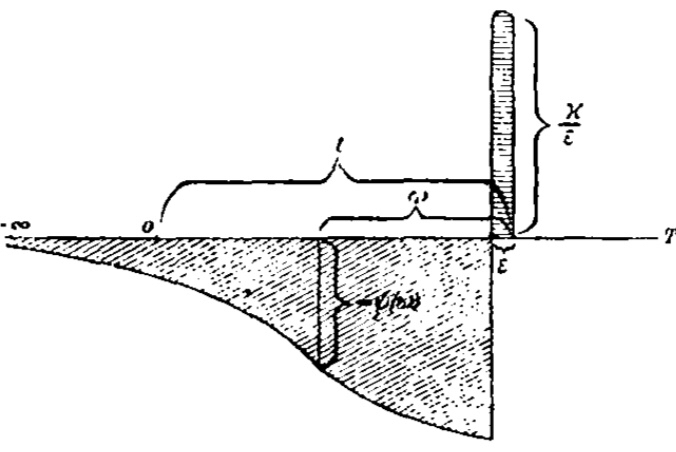
\includegraphics[width=150pt]{fig1}
\end{center}
\end{figure}

\begin{figure}
\begin{center}
	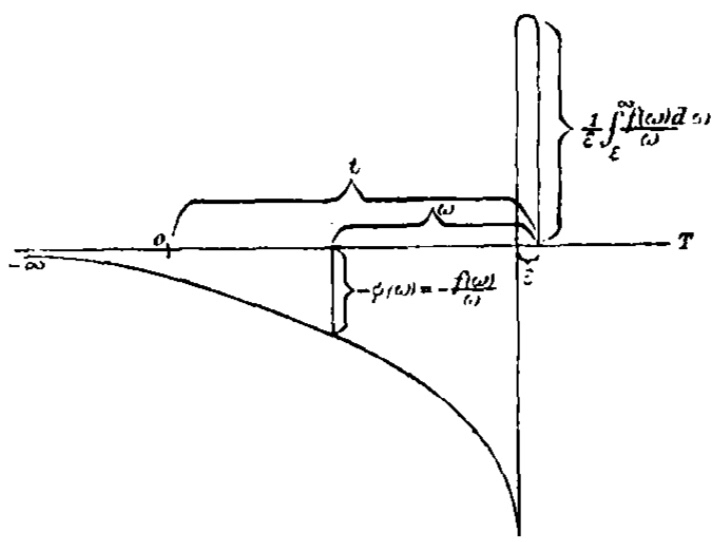
\includegraphics[width=150pt]{fig2}
\end{center}
\end{figure}

If the horizontally-shaded area is equal to the diagonally-shaded area, then the equations for the two cases approach those for a \?{viscous}{reibende} fluid, first if the whole shaded surface vanishes up to the part which has too-small values of $\omega$, second, if the motion happens very slowly. If the areas are not equal, then in these cases the equations approach those of Neumann-O.E.Meyer for the internal \?{friction}{Reibung} of fixed bodies.

In the special case that
\uequ{
N_1 &= \lambda\theta + 2\mu\ddx{u} - 
\alpha\lambda\int\limits_0^\infty\D\omega \exp{-b\omega}\theta(t-\omega) - 
a\mu\int\limits_0^\infty\D\omega\exp{-b\omega}\ddx{u(t-\omega)}\\
T_1 &= \mu p - a\mu\int\limits_0^\infty\D\omega \exp{-b\omega}p(t-\omega),
}
it is found that
\uequ{
bN_1 + \ddt{N_1} &= \lambda_1\theta + \mu_1\ddx{u} + \lambda\ddt{\theta} + 2\mu\ddX{u}\dY{x}\dY{t}\\
bT_1 + \ddt{T_1} &= \mu_1 p + \mu\ddt{p}
}
where $\lambda_1 = \lambda(b-\alpha)$, $\mu_1 = \mu(b-a)$ so
\uequ{
\varrho\left(b\ddX{u}\ddY{t} + \frac{\d{}^3 u}{\d{t}}\right)
= (\lambda_1 + \mu_1)\ddx{\theta} + \gamma_1\Delta u + (\lambda + \mu)\ddX{\theta}\dY{x}\dY{t} + \mu \ddt{\Delta}.
}
If $\gamma_1=0$, the two earlier shaded areas are equal. In the case that $\lambda_1=0$ as well, where of course \WTF{cubic compression} would also find no opposition after sufficiently long time, but in all cases where $\theta=0$ this equation can be integrated over $t$ and it  gives
\uequ{
\varrho b \ddt{u} + \varrho \ddX{u}\ddY{t} = 
(\lambda + \mu)\theta + \mu\Delta u
}
so for $\lambda+\mu=0$ (quasistability) but also in all cases where $\theta=0$, the equatiom of the electromagnetic theory of light for \WTF{semiconductors}. So here one obtains the term $\varrho b \d{u}/\d{t}$ which usually denotes one of the velocity-dependent forces in a totally different manner.

Munich, October 1892

\end{paper}
